\subsection{Training, Results, and Discussion}

The code for the training can be found in the notebook: \href{https://github.com/nicholaspun/IZ-Net/blob/master/notebooks/FaceDetection.ipynb}{\inlinecode{FaceDetection.ipynb}}.
We were, unfortunately, only able to achieve around $\sim25\%$ accuracy for our test set.
Sample outputs can be found in \Cref{Figure:Face-Detection:training:outputs-good} and \Cref{Figure:Face-Detection:training:outputs-bad}

\begin{figure}[htbp]
    \centering
    \begin{subfigure}{0.495\textwidth}
        \centering
        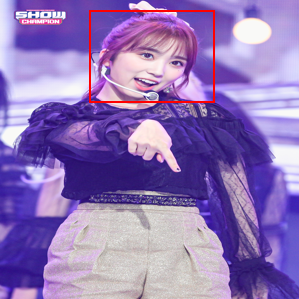
\includegraphics[width=0.6\textwidth]{images/faceDetec/training/result-1.png}
    \end{subfigure}
    \hfill
    \begin{subfigure}{0.495\textwidth}
        \centering
        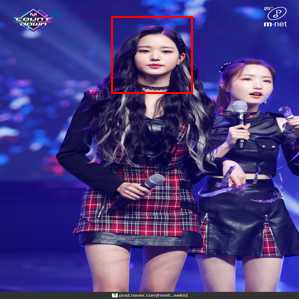
\includegraphics[width=0.6\textwidth]{images/faceDetec/training/result-2.png}
    \end{subfigure}
    \caption{
        2 decent outputs of our face detection model
    }
    \label{Figure:Face-Detection:training:outputs-good}
\end{figure}

\begin{figure}[htbp]
    \centering
    \begin{subfigure}{0.495\textwidth}
        \centering
        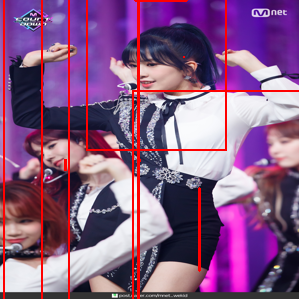
\includegraphics[width=0.6\textwidth]{images/faceDetec/training/result-3.png}
    \end{subfigure}
    \hfill
    \begin{subfigure}{0.495\textwidth}
        \centering
        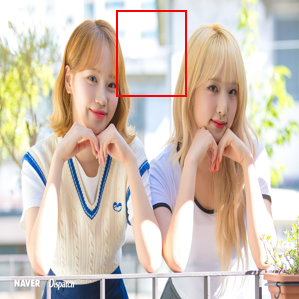
\includegraphics[width=0.6\textwidth]{images/faceDetec/training/result-4.png}
    \end{subfigure}
    \caption{
        2 not-so-decent outputs of our face detection model.
    }
    \label{Figure:Face-Detection:training:outputs-bad}
\end{figure}

On testing on images outside our training set (we lacked a validation set again here), there is also evidence of poor generalization of the model.
For example, in \Cref{Figure:Face-Detection:training:bad-generalization}, the bounding boxes completely miss the desired target.

\begin{figure}[htbp]
    \centering
    \begin{subfigure}{0.495\textwidth}
        \centering
        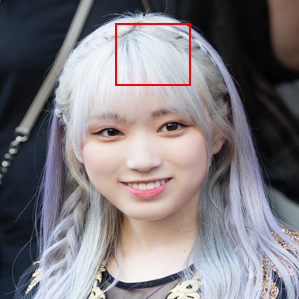
\includegraphics[width=0.6\textwidth]{images/faceDetec/training/bad-generalization.png}
    \end{subfigure}
    \hfill
    \begin{subfigure}{0.495\textwidth}
        \centering
        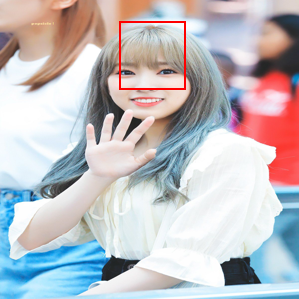
\includegraphics[width=0.6\textwidth]{images/faceDetec/training/bad-generalization-2.png}
    \end{subfigure}
    \caption{
        Evidence of bad generalization of our face detection model
    }
    \label{Figure:Face-Detection:training:bad-generalization}
\end{figure}

So, what happened?
We think there are several things at play here:
\begin{enumerate}[left=0pt]
\item \bf{Unsuitable architecture}

We sort of dug a hole for ourselves when we made the note at the start of the section stating that the loss function was the key learning opportunity.
Though we still stand by that, in reality, if the main goal was achieving high accuracy in predictions, there has been quite a lot of development in using various models along with YOLO.
For example, MobileNet \cite{mobilenet} is a much compact and efficient structure with the goal of being able to be used in devices with less computational power.
There's also the use of ShuffleNet \cite{shufflenet} in detecting collapsed buildings \cite{shufflenetBuildings}.
As a tangent, we were actually tempted to use ShuffleNet since it creates some new building blocks that would have been fun to play around with.

The idea that the architecture was limiting us came from that training, even at very low learning rates (we went as far as $10^{-6}$), could not improve the accuracy.
There's a possibility that we may have been losing on finer features of the facial structure in using DarkNet-53, especially since the architecture is very deep.

\item \bf{Poor training set}

This alludes to both the issue of high bias and high variance in our model.
The distribution of our training set consisted of many images where the true bounding box would solely be in the upper middle of the image.
This makes sense since the head is naturally located there for human beings.
However, this forces the model to overfit to this particular location, making it quite difficult for it generalize when there are multiple faces to detect.
For example, we can see this in the right image of \Cref{Figure:Face-Detection:training:outputs-bad}, where instead of predicting two separate bounding boxes, we predict one in the middle.
The solution here is simply to provide more training images where multiple faces exist.

This also leads well to the other reason our training set was not the best.
The pre-trained model that we used tend to \it{also} miss detections when multiple faces were present!
This means that we have a lot erroneous labellings in our training set.
We note that this hypothesis is a bit more far-reaching, as models usually resilient to small errors, but we mention it here as there's a small possibility of it affecting our training.

Finally, our training set is extremely small (around 1000 images) and so this naturally leads to higher variance.

\item \bf{Erroneous loss function}

We still aren't $100\%$ confident with our loss function since it diverges a bit from other implementations we found.
There's a possibility that our function admits undesirable minima leading to the cap in accuracy. 
We have no idea where one would start in trying to figure this one out though.
Perhaps rewriting the code mathematically and going from there might help, but even then, we are grasping at straws here.

\end{enumerate}